%%
% This is an Overleaf template for presentations
% using the TUM Corporate Desing https://www.tum.de/cd
%
% For further details on how to use the template, take a look at our
% GitLab repository and browse through our test documents
% https://gitlab.lrz.de/latex4ei/tum-templates.
%
% The tumbeamer class is based on the beamer class.
% If you need further customization please consult the beamer class guide
% https://ctan.org/pkg/beamer.
% Additional class options are passed down to the base class.
%
% If you encounter any bugs or undesired behaviour, please raise an issue
% in our GitLab repository
% https://gitlab.lrz.de/latex4ei/tum-templates/issues
% and provide a description and minimal working example of your problem.
%%

\documentclass[
  german,            % define the document language (english, german)
  aspectratio=169,    % define the aspect ratio (169, 43)
  % handout=2on1,       % create handout with multiple slides (2on1, 4on1)
  % partpage=false,     % insert page at beginning of parts (true, false)
  % sectionpage=true,   % insert page at beginning of sections (true, false)
]{tumbeamer}


% load additional packages
\usepackage{booktabs}
\usepackage{graphicx}
\usepackage{tikz}
\usepackage{url}
\usepackage{pgfplots}
\usepackage{hyperref}
\usepackage{pmboxdraw}
\usepackage{float}
\usepackage{listings}

% image path
\graphicspath{ {./resources/} }

% presentation metadata
\title{Übung 03: Unterprogramme und \\ Speicherzugriffe}
\subtitle{Einführung in die Rechnerarchitektur}
\author{Niklas Ladurner}

\institute{\theChairName\\\theDepartmentName\\\theUniversityName}
\date[\today]{\today}

\footline{\insertauthor~|~\insertshorttitle~|~\insertshortdate}


% macro to configure the style of the presentation
\TUMbeamersetup{
  title page = TUM tower,         % style of the title page
  part page = TUM toc,            % style of part pages
  section page = TUM toc,         % style of section pages
  content page = TUM more space,  % style of normal content pages
  tower scale = 1.0,              % scaling factor of TUM tower (if used)
  headline = TUM threeliner,      % which variation of headline to use
  footline = TUM default,         % which variation of footline to use
  % configure on which pages headlines and footlines should be printed
  headline on = {title page},
  footline on = {every page, title page=false},
}

% available frame styles for title page, part page, and section page:
% TUM default, TUM tower, TUM centered,
% TUM blue default, TUM blue tower, TUM blue centered,
% TUM shaded default, TUM shaded tower, TUM shaded centered,
% TUM flags
%
% additional frame styles for part page and section page:
% TUM toc
%
% available frame styles for content pages:
% TUM default, TUM more space
%
% available headline options:
% TUM empty, TUM oneliner, TUM twoliner, TUM threeliner, TUM logothreeliner
%
% available footline options:
% TUM empty, TUM default, TUM infoline


\begin{document}

\maketitle

\begin{frame}[c]{}{}
  \begin{center}
    \LARGE  Keine Garantie für die Richtigkeit der Tutorfolien: Bei Unklarheiten/Unstimmigkeiten 
    haben VL/ZÜ-Folien Recht!
  \end{center}
\end{frame}

\begin{frame}[c]{Sprünge und Unterprogramme}{}
  \begin{itemize}
    \item if, while, for $\rightarrow$ umgesetzt durch Sprünge
    \item jumps: unbedingt, branches: bedingt
    \item in x86 über Flags-Register, in RISC-V direkt im Befehl eingebaut
    \item Unterprogrammaufrufe: Sicherung, Parameter, Sprung + Rückkehr
  \end{itemize}
\end{frame}

\begin{frame}[c]{Caller- und Callee-saved Register}{}
  \begin{figure}[h]
  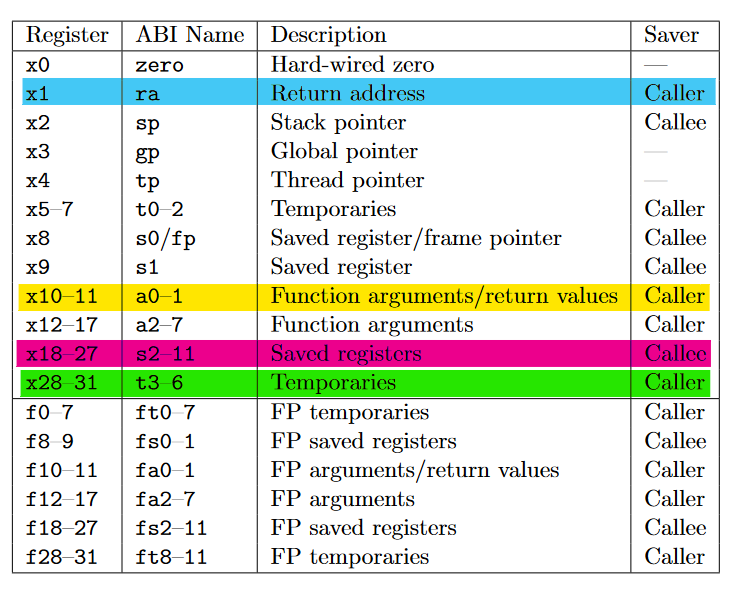
\includegraphics[height=0.75\textheight]{resources/w03_calling_conv_regs.png}
  \caption{Übersicht über die RISC-V-Register}
  \end{figure}
\end{frame}

\begin{frame}[c]{Von-Neumann-Architektur}{}
  \begin{figure}[h]
    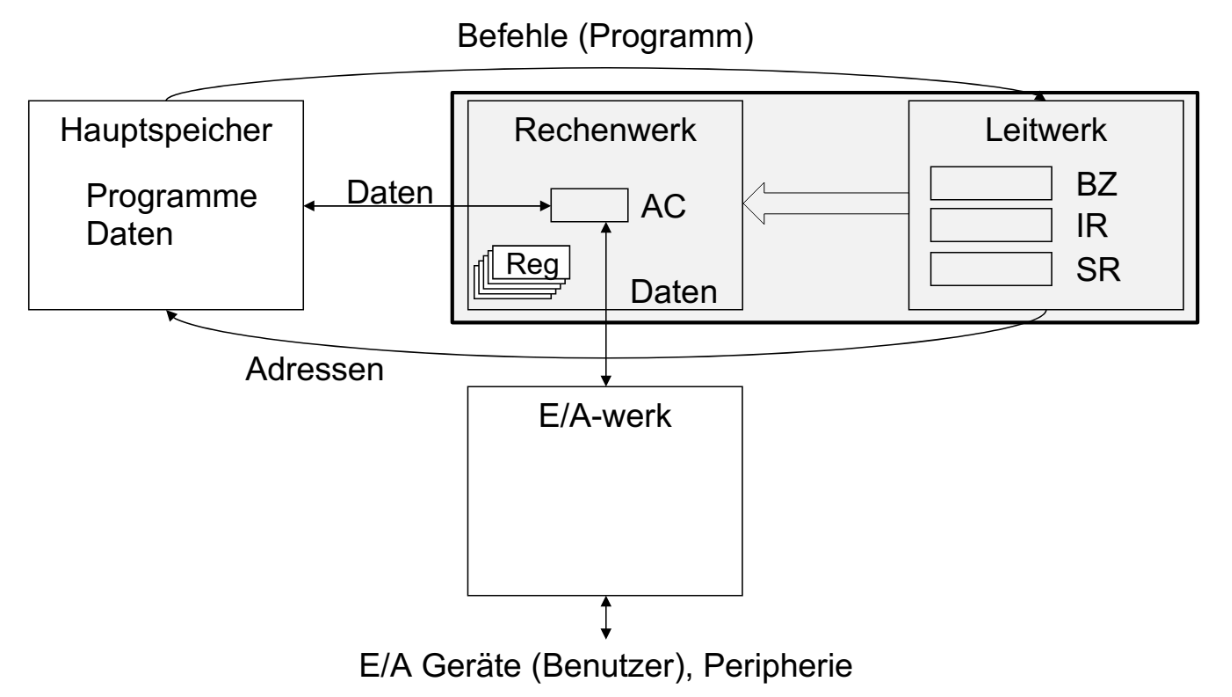
\includegraphics[height=0.75\textheight]{resources/w03_von_Neumann.png}
    \caption{Schematische Darstellung der von-Neumann-Architektur}
  \end{figure}
\end{frame}

\begin{frame}[fragile, c]{Hauptspeicher}{}
  \begin{itemize}
    \item Hauptspeicher = RAM, nicht Festplatten etc.
    \item Laden/speichern mittels lb/sb/lw/sw
    \item Register als Basisadresse + Offset
  \end{itemize}  
\end{frame}

\begin{frame}[fragile, c]{Speicherzugriffe in RISC-V}{}
  lade 32 Bit an der Adresse a0 + 0 Bytes Offset in das Register t0: 
  \begin{verbatim}lw t0, 0(a0)\end{verbatim}
  lade 8 Bit an der Adresse a2 - 4 Bytes Offset in das Register t1: 
  \begin{verbatim}lb t1, -4(a2)\end{verbatim}
  speichere den gesamten Inhalt des Registers t2 an die Adresse a1 + 16 Bytes Offset:
  \begin{verbatim}sw t2, 16(a1)\end{verbatim}
\end{frame}

\begin{frame}[c]{}{}
  \begin{center}
    \LARGE Fragen?\\
    \Large (Die ZÜ-Folien sind sehr gut, schaut euch die an)
  \end{center}
\end{frame}

\begin{frame}[c]{Artemis-Hausaufgaben}{}
  \begin{itemize}
    \item H03 - Palindrom bis 12.11.2023 23:59 Uhr
    \item Speicheroperationen
    \item lasst euch nicht vom Label 'hard' abschrecken, das Prinzip ist sehr simpel
  \end{itemize}
\end{frame}

\begin{frame}[fragile, c]{Links}{}
  \begin{itemize}
    \item Zulip: \href{https://zulip.in.tum.de/#narrow/stream/1917-ERA-Tutorium---Mi-1600-MI4}{\glqq ERA Tutorium - Mi-1600-MI4\grqq}
    bzw. \href{https://zulip.in.tum.de/#narrow/stream/1940-ERA-Tutorium---Fr-1100-MW2}{\glqq ERA Tutorium - Fr-1100-MW2\grqq}
    \item \href{https://riscv.org/wp-content/uploads/2017/05/riscv-spec-v2.2.pdf}{RISC-V-Spezifikation}
    \item \href{https://www.geeksforgeeks.org/computer-organization-von-neumann-architecture/}{Von-Neumann-Architektur}
    \item \href{https://msyksphinz-self.github.io/riscv-isadoc/html/rvi.html}{übersichtlichere Instruktionsliste}
  \end{itemize}
\end{frame}

\maketitle

\end{document}
